\newcommand{\posterRhic}[1]{

\setlength{\frameWidth}{#1}
\setlength{\unitlength}{0.02\frameWidth}
\psset{unit=\unitlength}

\rput[lb](1,-1){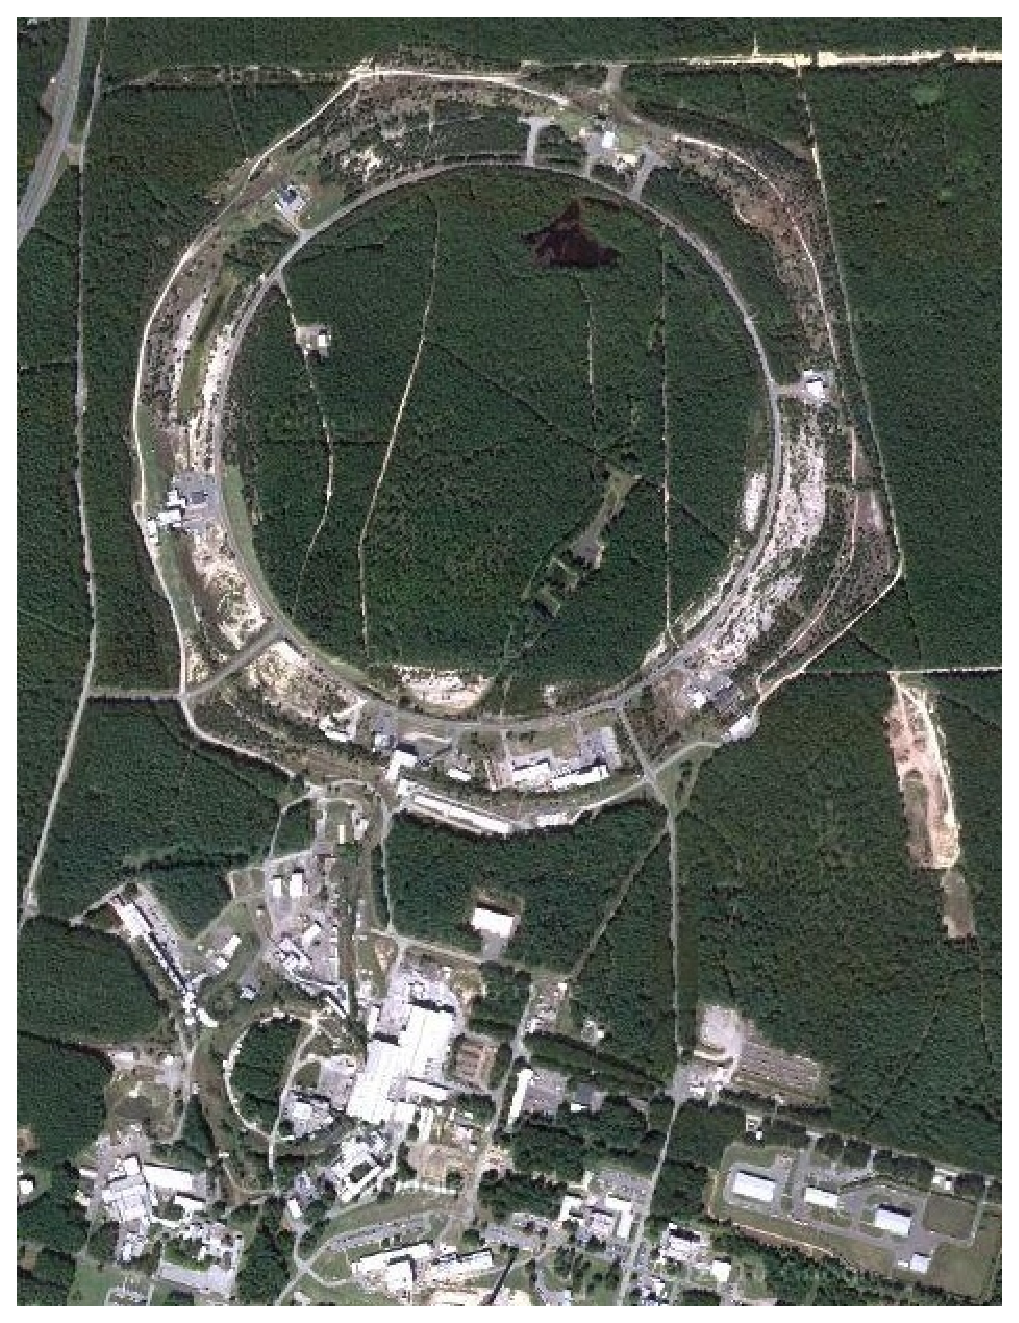
\includegraphics[width=24\unitlength]{graphics/areal}}

\psarc[linewidth=0.35, arrowscale=2, linecolor=blueLight, fillstyle=none]{<-}(12.6,20.2){6.2}{-20}{60}
\psarc[linewidth=0.35, arrowscale=2, linecolor=yellow, fillstyle=none]{->}(12.6,20.2){6.2}{160}{240}

\rput(17,19){\textcolor{blueLight}{\LARGE \boldmath $p$}}
\rput(10,17){\textcolor{yellow}{\LARGE \boldmath $p$}}

\rput[lt](26.5,29) {%
\begin{minipage}{24\unitlength}

\raggedright

\begin{list}{\labelitemi}{\setlength{\itemsep}{0mm}
                          \setlength{\topsep}{0mm}
                          \setlength{\leftmargin}{0mm}
                          \setlength{\rightmargin}{0mm}}

   \item \textbf{RHIC is the largest scientific tool at BNL}

   \begin{list}{\labelitemii}{\setlength{\itemsep}{5mm}}

       \item Ring diameter is $\approx 0.75$~miles

        \item Accelerates subatomic particles \textbf{\small protons, deuterons, Si, Cu,
        Au, U}\\
        to nearly the speed of light

      \item Collides particles head-on at two interaction points
   \end{list}


    \item \textbf{RHIC is the first and only world's polarized collider}

   \begin{list}{\labelitemii}{\setlength{\itemsep}{5mm}}
        \item In operation since 2000
        \item Improving performance from year to year
   \end{list}

\end{list}

\end{minipage}
}

%\rput{0}{\psgrid[gridlabels=0.7,subgriddiv=0, griddots=3](1,-1)(0,0)(\myPsPictureWidthLocal,\myPsPictureHeightLocal)}

}

\setlength{\unitlength}{10mm}
\psset{unit=\unitlength}
